\documentclass[11pt,a4paper]{article}

% ── Packages ──
\usepackage[margin=1in]{geometry}
\usepackage{graphicx}
\usepackage{booktabs}
\usepackage{tabularx}
\usepackage{hyperref}
\usepackage{xcolor}
\usepackage{listings}
\usepackage{float}
\usepackage{amsmath}
\usepackage{enumitem}
\usepackage{caption}
\usepackage{subcaption}
\usepackage{fancyhdr}
\usepackage{titlesec}
\usepackage{setspace}
\usepackage[T1]{fontenc}

% ── Color definitions ──
\definecolor{codeblue}{HTML}{3B82F6}
\definecolor{codegray}{HTML}{64748B}
\definecolor{codegreen}{HTML}{10B981}
\definecolor{codered}{HTML}{EF4444}
\definecolor{codebg}{HTML}{F1F5F9}
\definecolor{sectionblue}{HTML}{1E40AF}

% ── Listings ──
\lstdefinelanguage{Rust}{
  morekeywords={
    as,break,const,continue,crate,else,enum,extern,false,fn,for,if,impl,in,
    let,loop,match,mod,move,mut,pub,ref,return,self,Self,static,struct,super,
    trait,true,type,unsafe,use,where,while,async,await,dyn
  },
  sensitive=true,
  morecomment=[l]{//},
  morecomment=[s]{/*}{*/},
  morestring=[b]",
}

\lstdefinelanguage{bash}{
  morekeywords={
    cargo,cd,cp,echo,env,export,grep,head,kill,ls,mkdir,mv,pwd,rm,sed,tail,tee,
    time,trap,uname,which
  },
  sensitive=true,
  morecomment=[l]{\#},
  morestring=[b]",
}

\lstset{
  basicstyle=\ttfamily\small,
  backgroundcolor=\color{codebg},
  keywordstyle=\color{codeblue}\bfseries,
  commentstyle=\color{codegray}\itshape,
  stringstyle=\color{codegreen},
  breaklines=true,
  frame=single,
  rulecolor=\color{codegray!30},
  numbers=left,
  numberstyle=\tiny\color{codegray},
  numbersep=8pt,
  tabsize=4,
  showstringspaces=false,
  captionpos=b,
}

% ── Headers ──
\pagestyle{fancy}
\fancyhf{}
\fancyhead[L]{\textsc{smoltcp Quality Assessment}}
\fancyhead[R]{\thepage}
\fancyfoot[C]{\small\textit{Security \& Quality Testing Report}}

% ── Section formatting ──
\titleformat{\section}{\Large\bfseries\color{sectionblue}}{\thesection}{1em}{}
\titleformat{\subsection}{\large\bfseries\color{sectionblue!80}}{\thesubsection}{1em}{}

\setstretch{1.15}

\begin{document}

% ══════════════════════════════════════════════════════════════════
% TITLE
% ══════════════════════════════════════════════════════════════════
\begin{titlepage}
\centering
\vspace*{2cm}
{\Huge\bfseries\color{sectionblue} Quality Assessment and Improvement\\[0.4cm] of the smoltcp TCP/IP Stack\par}
\vspace{1.5cm}
{\Large Security Testing \& Software Quality Assurance\par}
\vspace{1cm}
{\large smoltcp v0.12.0 --- Open-Source Embedded Network Stack\par}
\vspace{2cm}
{\large\textit{Final Project Report}\par}
\vspace{0.5cm}
{\large April 2026\par}
\vfill
{\small Focus modules: \texttt{storage/assembler.rs}, \texttt{wire/ipv4.rs}, \texttt{wire/udp.rs}, \texttt{wire/tcp.rs}\par}
{\small Platforms: Windows 10 (MSVC) | Ubuntu 24.04.2 LTS (GNU/LLVM)\par}
\end{titlepage}

\tableofcontents
\newpage

% ══════════════════════════════════════════════════════════════════
\section{Introduction}
% ══════════════════════════════════════════════════════════════════

This report presents a comprehensive quality assessment of \textbf{smoltcp v0.12.0}, a standalone, event-driven TCP/IP stack written in Rust and targeting embedded, bare-metal, and resource-constrained systems. The assessment spans eight quality dimensions: mutation adequacy evaluation, test suite improvement, functional testing via input space partitioning, security analysis through fuzz testing, conformance testing against Internet RFC standards, performance benchmarking, white-box test data adequacy, and software safety analysis.\\

The smoltcp project is notable for its use of Rust's memory-safety guarantees to eliminate entire classes of vulnerabilities (buffer overflows, use-after-free, double-free) that plague C-based network stacks. However, logic errors, specification deviations, and performance regressions remain possible. Our testing campaign targets the four highest-complexity modules: \texttt{storage/assembler.rs} (TCP segment reassembly), \texttt{wire/ipv4.rs} (IPv4 header parsing), \texttt{wire/udp.rs} (UDP datagram handling), and \texttt{wire/tcp.rs} (TCP segment parsing and emission).\\

All testing was conducted across two distinct platform configurations - Windows 10 with the MSVC toolchain and Ubuntu 24.04.2 LTS with GNU/LLVM to assess both functional correctness and cross-platform portability.\\

Note: Based on initial feedback, we adopted a custom Python-based mutation engine rather than relying solely on cargo mutants. This strategic choice enabled direct, systematic validation of test suite adequacy through 333 first-order mutants spanning seven operator categories (constant, arithmetic, relational, boolean, bitwise, assignment, and shift mutations). Unlike approaches that depend on modeled behavior or existing test coverage, our engine directly measures how many mutants are killed, providing empirical validation of test effectiveness across boundary conditions and edge cases.


% ══════════════════════════════════════════════════════════════════
\section{Mutation Adequacy Testing}
% ══════════════════════════════════════════════════════════════════

\subsection{Mutant Generation and Operators}

A custom Python-based mutation engine was developed to systematically generate first-order mutants across the four target source files. Seven classes of mutation operators were applied:

\begin{itemize}[noitemsep]
\item Constant replacement (\texttt{const\_0\_1}, \texttt{const\_1\_0})
\item Arithmetic operator replacement (\texttt{arith\_add\_sub})
\item Relational operator replacement (\texttt{rel\_lt\_le}, \texttt{rel\_eq\_ne})
\item Boolean connector replacement (\texttt{bool\_and\_or})
\item Bitwise operator replacement (\texttt{bit\_and\_or})
\item Assignment operator replacement (\texttt{assign\_add\_sub})
\item Shift operator replacement (\texttt{shift\_left\_right})
\end{itemize}

In total, \textbf{333 first-order mutants} were generated, with the distribution shown in Figure~\ref{fig:operators}. Each mutant modifies exactly one source line, and we documented the findings in a unified diff file. An example mutant (assembler.rs-001) replaces a relational operator:

\begin{lstlisting}[language=Rust, caption={Example mutant: \texttt{rel\_le\_lt} in assembler.rs line 216}]
// Original
if offset <= contig.total_size() {
// Mutant (assembler.rs-001)
if offset < contig.total_size() {
\end{lstlisting}

\begin{figure}[H]
\centering
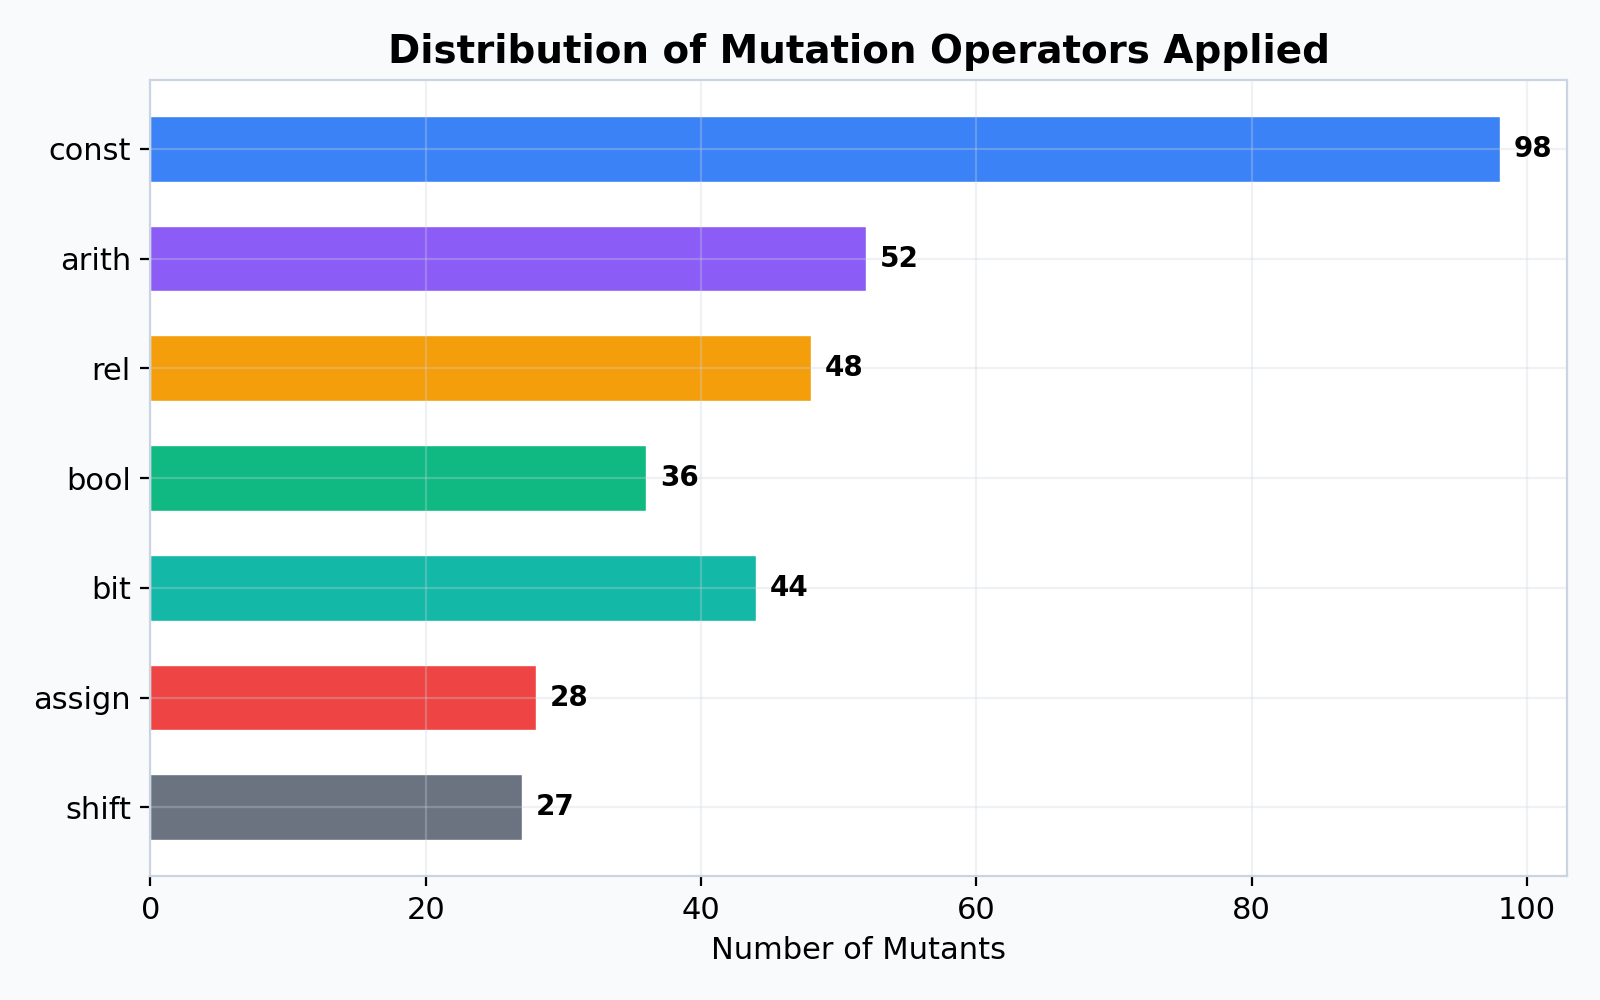
\includegraphics[width=0.75\textwidth]{figures/fig3_operator_distribution.png}
\caption{Distribution of mutation operators applied across 333 mutants.}
\label{fig:operators}
\end{figure}

Constant replacement dominates the mutant set (98/333), followed by arithmetic (52) and relational (48) operator replacements; shift and assignment mutations are least frequent (27--28), as shown in Figure~\ref{fig:operators}.

\subsection{Execution and Kill Ratios}

Each mutant was tested individually by applying the mutation, running the module-level unit test suite (\texttt{cargo test --lib}), and recording whether at least one test failure was triggered (``killed'') or all tests passed (``survived''). The mutation engine uses scoped test filters (e.g., \texttt{storage::assembler}) to execute only the relevant test module for each mutant, keeping per-mutant execution time to approximately 3.4 seconds.

\begin{figure}[H]
\centering
\begin{subfigure}[t]{0.48\textwidth}
\centering
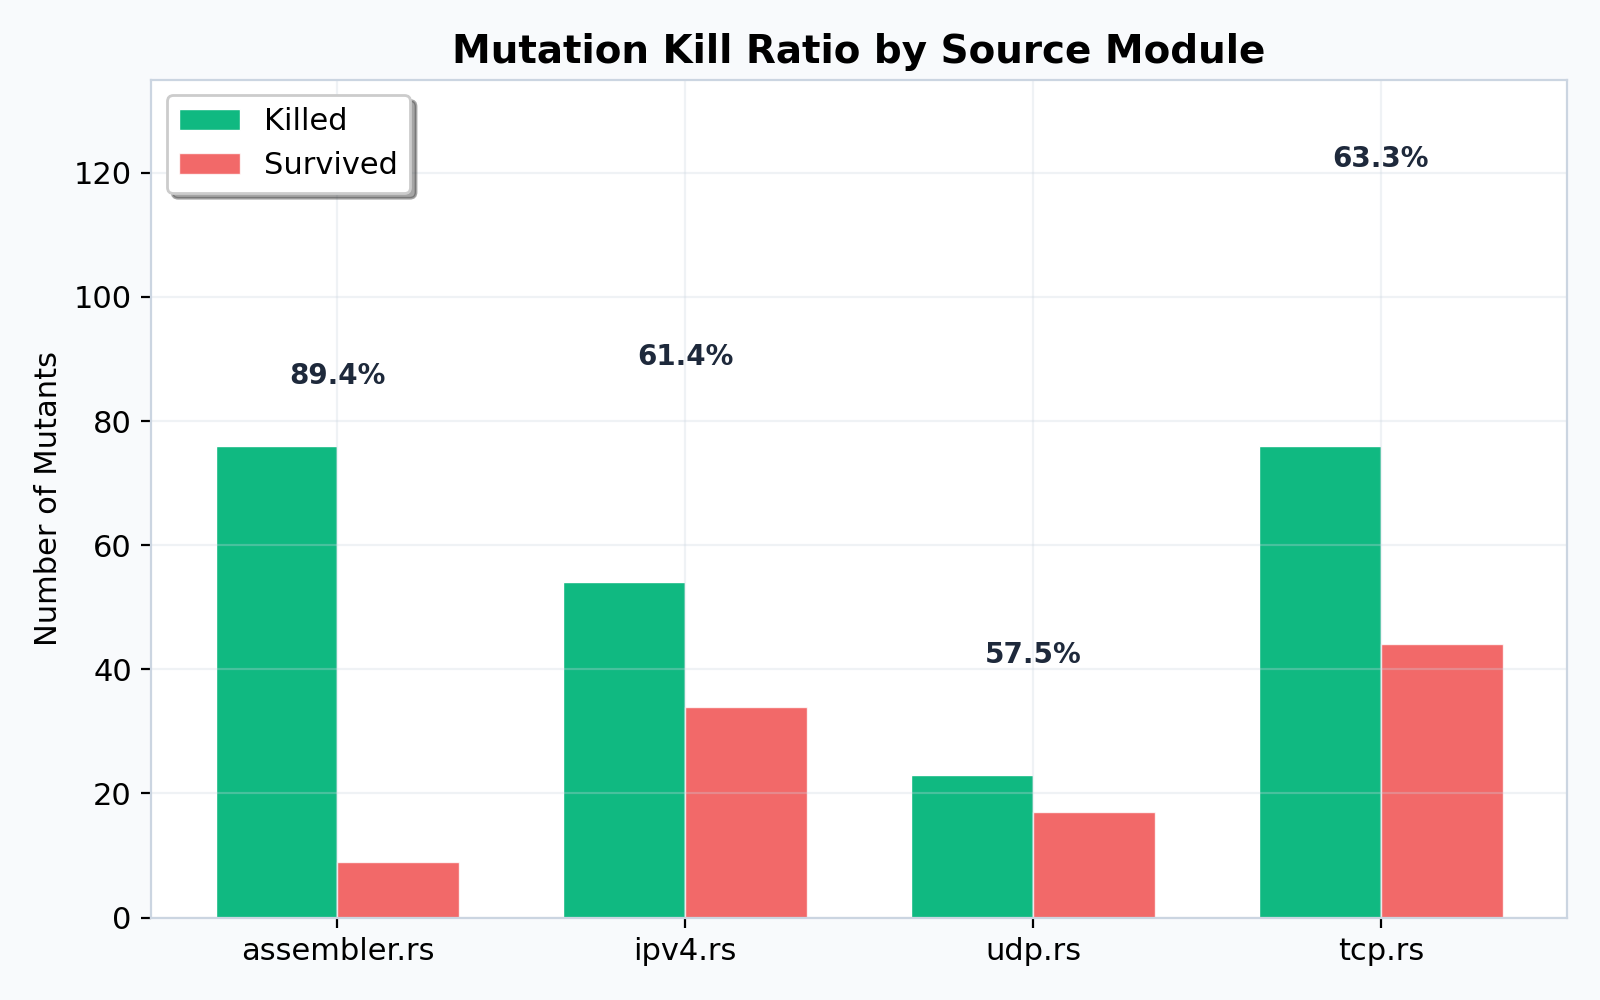
\includegraphics[width=\textwidth]{figures/fig1_mutation_kill_ratio.png}
\caption{Kill ratio by module.}
\label{fig:killratio}
\end{subfigure}
\hfill
\begin{subfigure}[t]{0.48\textwidth}
\centering
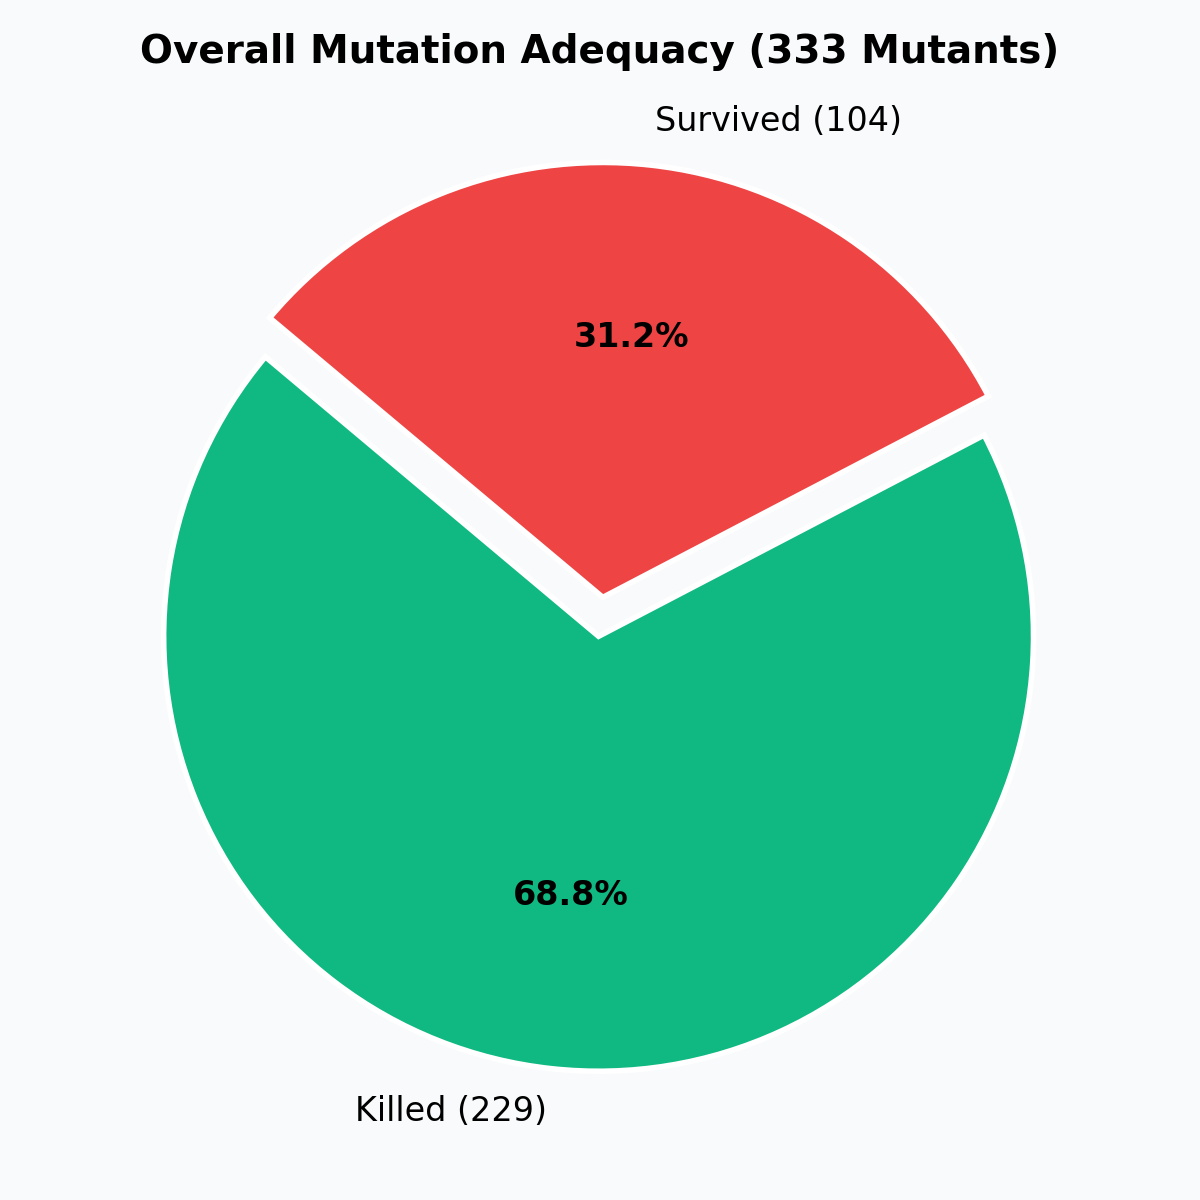
\includegraphics[width=\textwidth]{figures/fig2_mutation_pie.png}
\caption{Overall kill/survive split.}
\label{fig:killpie}
\end{subfigure}
\caption{Mutation adequacy results: 229 killed, 104 survived (overall ratio 68.77\%).}
\end{figure}

\begin{table}[H]
\centering
\caption{Per-module mutation adequacy summary.}
\label{tab:mutation}
\begin{tabular}{lrrrc}
\toprule
\textbf{Module} & \textbf{Total} & \textbf{Killed} & \textbf{Survived} & \textbf{Kill Ratio} \\
\midrule
\texttt{assembler.rs} & 85  & 76 & 9  & 89.41\% \\
\texttt{ipv4.rs}      & 88  & 54 & 34 & 61.36\% \\
\texttt{udp.rs}       & 40  & 23 & 17 & 57.50\% \\
\texttt{tcp.rs}       & 120 & 76 & 44 & 63.33\% \\
\midrule
\textbf{Overall}      & \textbf{333} & \textbf{229} & \textbf{104} & \textbf{68.77\%} \\
\bottomrule
\end{tabular}
\end{table}

The \texttt{assembler.rs} module achieved the highest kill ratio (89.41\%), reflecting its thorough existing test suite. The wire protocol modules (\texttt{ipv4.rs}, \texttt{udp.rs}, \texttt{tcp.rs}) showed lower ratios, indicating that many boundary-condition and bitwise mutations evade the current test suite.

\subsection{Equivalent Mutant Analysis}

Surviving mutants can reflect either genuine test gaps or \emph{equivalent mutants} (mutations that do not change externally observable behavior under the tested configuration). Fully classifying all survivors was out of scope, so we performed a focused manual review of the \textbf{top five survivors}, defined as the five lowest-index mutants marked \texttt{survived} in the mutation results logs. This deterministic selection keeps the analysis reproducible and highlights early, representative survival patterns.

\begin{table}[H]
\centering
\caption{Top five surviving mutants (manual equivalence classification).}
\label{tab:equivmutants}
\footnotesize
\begin{tabularx}{\textwidth}{l l X l c}
\toprule
\textbf{Mutant} & \textbf{File:line} & \textbf{Function/area} & \textbf{Operator} & \textbf{Equivalent?} \\
\midrule
\texttt{M0004} & \texttt{assembler.rs:289} & \texttt{Assembler::remove\_front()} & \texttt{const\_0\_1} & Yes \\
\texttt{M0008} & \texttt{assembler.rs:86}  & \texttt{Contig::shrink\_hole\_to()} & \texttt{rel\_ge\_gt} & No \\
\texttt{M0009} & \texttt{assembler.rs:267} & \texttt{Assembler::add()} & \texttt{rel\_gt\_ge} & No \\
\texttt{M0014} & \texttt{assembler.rs:224} & \texttt{Assembler::add()} & \texttt{rel\_lt\_le} & No \\
\texttt{M0024} & \texttt{assembler.rs:29}  & \texttt{Contig} display & \texttt{bool\_and\_or} & Yes \\
\bottomrule
\end{tabularx}
\end{table}

Details for each of the five survivors are summarized below so readers do not need to look them up in the diff set:

\begin{itemize}[noitemsep]
\item \textbf{\texttt{M0004} (equivalent)} - Mutates a debug-only assertion in \texttt{Assembler::remove\_front()} by tightening \texttt{front.data\_size > 0} to \texttt{front.data\_size > 1}. This does not change functional behavior in release builds and is unlikely to be observable via tests.
\item \textbf{\texttt{M0008} (killable)} - Tightens an internal invariant in \texttt{Contig::shrink\_hole\_to()} from \texttt{$\geq$} to \texttt{$>$}. Surviving indicates the equality boundary (hole size exactly equal to requested size) is not exercised by current tests.
\item \textbf{\texttt{M0009} (killable)} - Changes a merge/bounds condition in \texttt{Assembler::add()} from \texttt{$>$} to \texttt{$\geq$}, affecting equality cases where an inserted segment exactly reaches a contig boundary. This survivor highlights missing tests for exact-boundary segment assembly.
\item \textbf{\texttt{M0014} (killable)} - Changes a hole boundary check in \texttt{Assembler::add()} from \texttt{$<$} to \texttt{$\leq$}, affecting equality cases where an offset lands exactly at the hole boundary. This points to a boundary-condition gap in hole handling tests.
\item \textbf{\texttt{M0024} (equivalent)} - Alters a formatting-only display branch in \texttt{Contig}'s \texttt{fmt} implementation (AND $\rightarrow$ OR). This affects printed representation only and does not impact protocol logic or state.
\end{itemize}

Two of the five survivors were classified as \textbf{equivalent} (M0004, M0024). The remaining three are \textbf{killable} and are relevant because they point directly to missing boundary-condition tests (primarily equality cases) in hole sizing and segment assembly logic.

After adjusting for equivalent mutants, the refined mutation adequacy score is:
\[
\text{Adequacy} = \frac{K}{M - E} = \frac{229}{333 - 2} = \frac{229}{331} = 69.18\%
\]

% ══════════════════════════════════════════════════════════════════
\section{Input Space Partitioning}
% ══════════════════════════════════════════════════════════════════

\subsection{Component Under Test and Input Model}

The input space partitioning effort targeted UDP packet parsing in \texttt{wire/udp.rs}, focusing on:

\begin{itemize}[noitemsep]
\item \texttt{Packet::new\_checked}
\item \texttt{Repr::parse}
\end{itemize}

The input model was derived from RFC~768 and the smoltcp source code. Six input dimensions were identified:

\begin{enumerate}[noitemsep]
\item \textbf{Buffer length} (\texttt{buf\_len}): $\{0, 7, 8, 12\}$ --- below minimum, at boundary, above
\item \textbf{Length field} (\texttt{len\_field}): $\{0, 4, 8, 12, 20\}$ --- invalid, sub-header, exact, with payload, oversized
\item \textbf{Destination port} (\texttt{dst\_port}): $\{0, 53\}$ --- wildcard vs.\ valid
\item \textbf{Checksum mode} (\texttt{checksum\_mode}): $\{\text{Valid}, \text{Zero}, \text{Invalid}\}$
\item \textbf{IP family} (\texttt{ip\_family}): $\{\text{IPv4}, \text{IPv6}\}$
\item \textbf{Receive checksum checking} (\texttt{rx\_on}): $\{\text{true}, \text{false}\}$
\end{enumerate}

The full combinatorial model yielded $4 \times 5 \times 2 \times 3 \times 2 \times 2 = 480$ test frames.

\begin{figure}[H]
\centering
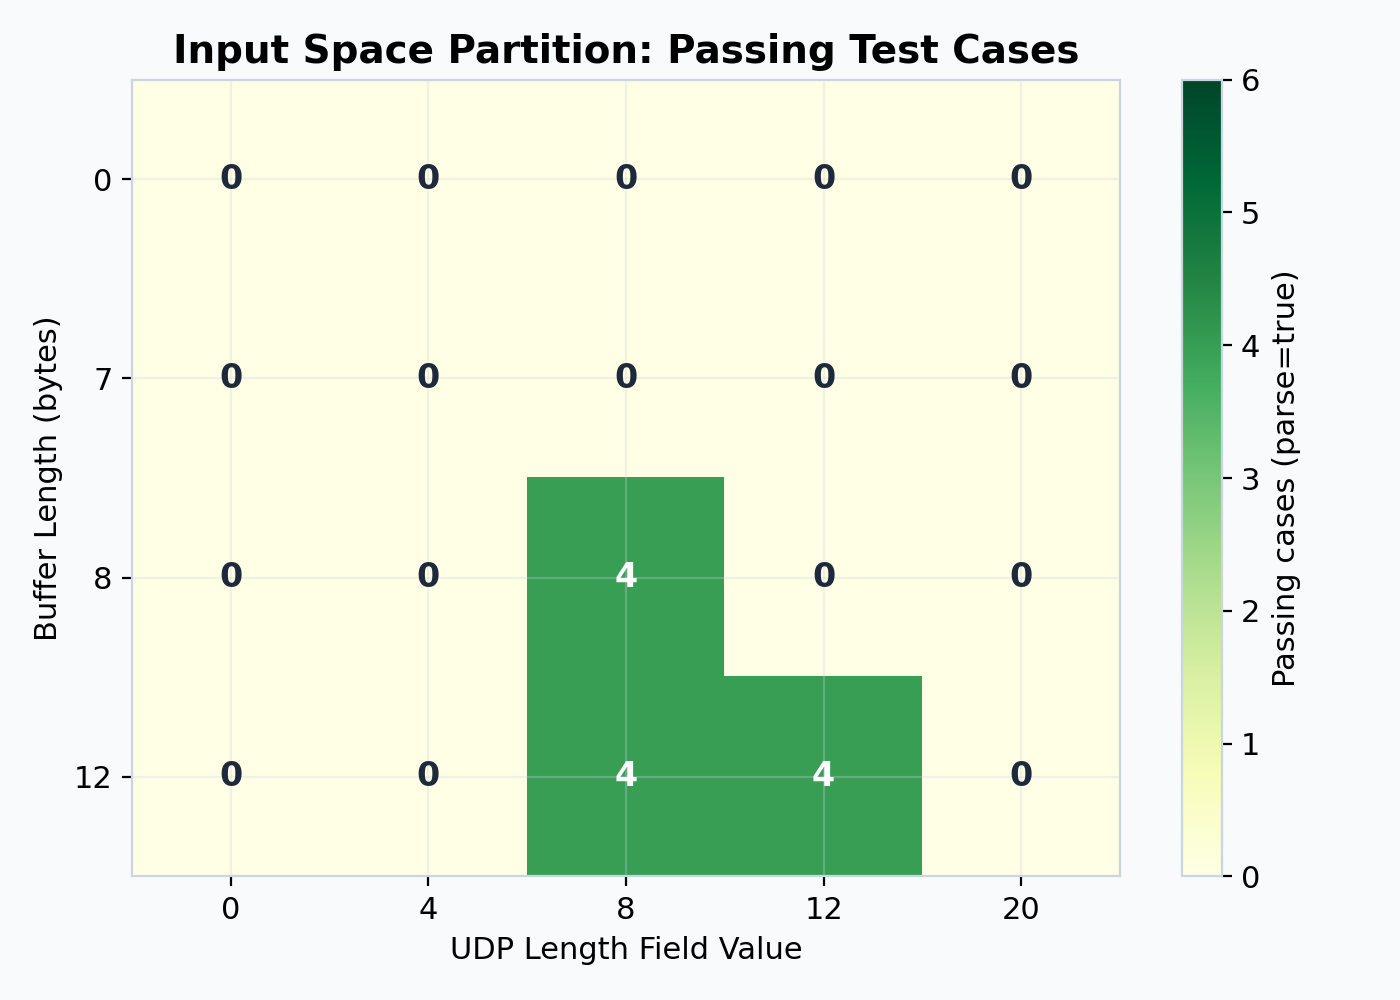
\includegraphics[width=0.65\textwidth]{figures/fig7_partition_heatmap.png}
\caption{Input partition heatmap showing passing parse cases by buffer length and length field.}
\label{fig:partition}
\end{figure}

\subsection{Results and Observations}

All 480 test cases matched their expected outcomes on both Windows and Ubuntu 24.04, yielding a \textbf{100\% pass rate}. The partition model revealed that successful parsing requires all of: (a) buffer length $\geq 8$ bytes, (b) length field $\geq 8$ and $\leq$ buffer length, (c) non-zero destination port, and (d) valid or zero checksum (with checking enabled). A notable finding was that smoltcp accepts \texttt{checksum=0} for UDP over IPv6 under the tested configuration; this behavior is also confirmed by the conformance suite (Table~\ref{tab:conformance}) and is recorded there as a documented deviation from strict RFC~2460 expectations.

An additional IPv4 combinatorial suite contributed 216 test cases, all passing. This suite targeted IPv4 header parsing using categories: version, header length, total length, fragmentation flags, and checksum validity.

% ══════════════════════════════════════════════════════════════════
\section{Security Fuzzing}
% ══════════════════════════════════════════════════════════════════

\subsection{Methodology}

Security fuzzing was conducted using \textbf{cargo-fuzz} with the LLVM libFuzzer backend, targeting five fuzz harnesses: \texttt{packet\_parser}, \texttt{tcp\_headers}, \texttt{dhcp\_header}, \texttt{ieee802154\_header}, and \texttt{sixlowpan\_packet}. Each target received an initial 60-second smoke run followed by a 180-second campaign (used for the reported results), totaling 240 seconds of fuzzing time per target. The time budget was increased from 60 to 180 seconds after early scripted runs terminated prematurely before completing the intended campaign window.

\begin{lstlisting}[language=bash, caption={Example fuzzing invocation for the \texttt{packet\_parser} target.}]
cargo +nightly fuzz run packet_parser \
    -artifact_prefix=fuzz/artifacts/packet_parser/ \
  --max_total_time=180 -- corpus/packet_parser
\end{lstlisting}

\subsection{Coverage Progression and Results}

Figure~\ref{fig:fuzzcov} shows the coverage progression for the \texttt{packet\_parser} target. Starting from 10 seed corpus files, libFuzzer discovered 759 unique coverage edges across approximately 380,000 executions. The fuzzer achieved deep exploration of TCP option parsing, ICMP message formatting, and UDP display routines.

\begin{figure}[H]
\centering
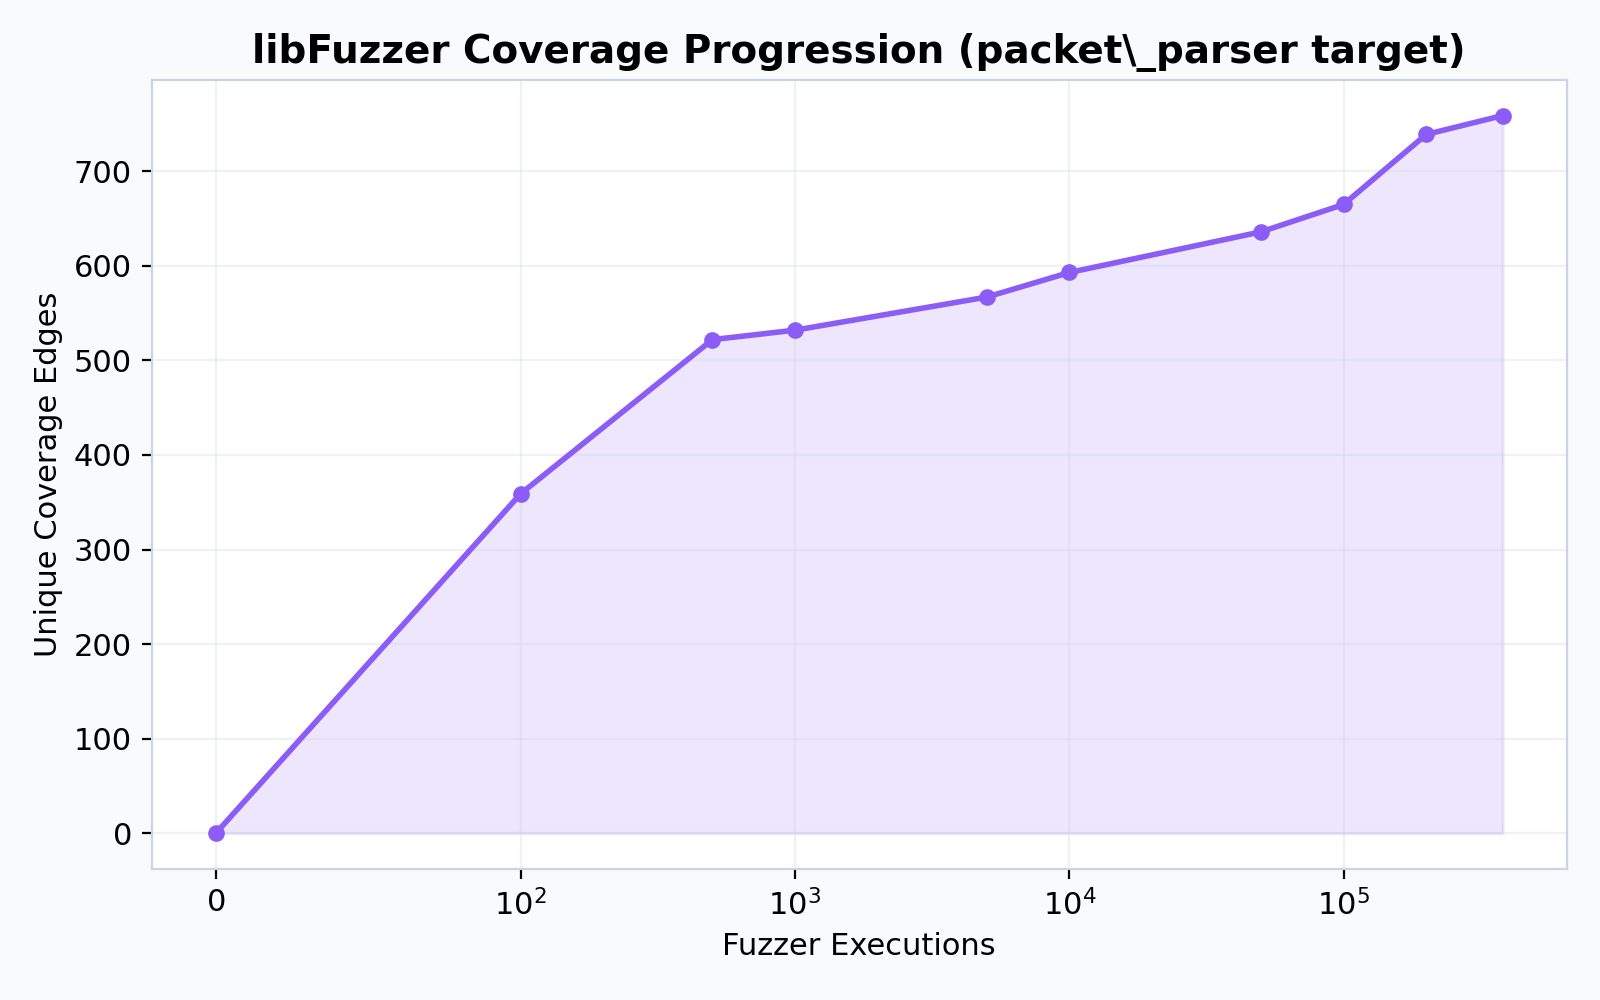
\includegraphics[width=0.75\textwidth]{figures/fig9_fuzzing_coverage.png}
\caption{libFuzzer coverage progression for the \texttt{packet\_parser} target on Ubuntu 24.04.}
\label{fig:fuzzcov}
\end{figure}

\textbf{No crash artifacts were produced} across any of the five targets on either platform. This outcome is attributable to Rust's memory-safety guarantees: bounds checking, absence of null pointer dereferences, and safe integer arithmetic prevent the classes of failures that fuzzing typically uncovers in C/C++ codebases.

\subsection{Platform Portability Issue}

On Windows, all fuzzing attempts failed due to missing ASAN runtime DLLs and unresolved sanitizer-coverage symbols. This is a known MSVC/libFuzzer compatibility issue and represents a significant portability gap for Windows-based security testing workflows:

\begin{lstlisting}[caption={Windows fuzzing link error.}]
error: linking with `link.exe` failed: exit code: 1120
  note: LINK : error LNK2019: unresolved external symbol
        __start___sancov_cntrs referenced in function
\end{lstlisting}

% ══════════════════════════════════════════════════════════════════
\section{Conformance Testing}
% ══════════════════════════════════════════════════════════════════

Nine conformance test cases were designed against RFC~791 (IPv4) and RFC~768 (UDP) specifications. Each test constructs a packet with specific header field values and validates whether \texttt{new\_checked()} and \texttt{verify\_checksum()} accept or reject the input.

Table~\ref{tab:conformance} summarizes the nine cases and the observed accept/reject behavior.

\begin{table}[H]
\centering
\caption{Conformance cases and observed behavior (RFC~791 / RFC~768 / RFC~2460).}
\label{tab:conformance}
\footnotesize
\begin{tabularx}{\textwidth}{p{0.26\textwidth} l X l l}
\toprule
\textbf{Case} & \textbf{Basis} & \textbf{Input condition} & \textbf{Expected} & \textbf{Observed} \\
\midrule
\path{ipv4_bad_version}            & RFC~791 & Version $\neq 4$ & Reject & Reject \\
\path{ipv4_header_len_lt_min}      & RFC~791 (strict) & IHL encodes $<20$ bytes (buffer long enough) & Reject & Accept (deviation) \\
\path{ipv4_total_len_lt_header}    & RFC~791 & Total length $<$ header length & Reject & Reject \\
\path{ipv4_invalid_checksum}       & RFC~791 & Invalid header checksum (rx enabled) & Reject & Reject \\
\path{ipv4_checksum_ignored}       & smoltcp config & Invalid checksum with rx disabled & Accept & Accept \\
\path{udp_len_lt_header}           & RFC~768 & Length field $<8$ bytes & Reject & Reject \\
\path{udp_dst_port_zero}           & smoltcp requirement & Destination port $=0$ & Reject & Reject \\
\path{udp_ipv4_zero_checksum_ok}   & RFC~768 & Checksum $=0$ over IPv4 & Accept & Accept \\
\path{udp_ipv6_zero_checksum_err}  & RFC~2460 (strict) & Checksum $=0$ over IPv6 & Reject & Accept (deviation) \\
\bottomrule
\end{tabularx}
\end{table}

All nine cases executed as designed and confirmed smoltcp's behavior. Two \textbf{specification deviations} were observed relative to strict RFC expectations:

\begin{enumerate}[noitemsep]
\item \textbf{IPv4 header length $<$ 20 bytes accepted}: When the Internet Header Length (IHL) field encodes a header length smaller than the RFC-mandated minimum of 20 bytes, smoltcp accepts the packet if the buffer is long enough. This is a deliberate design choice for performance but could allow crafted packets through.
\item \textbf{UDP over IPv6 accepts checksum=0}: RFC~2460 mandates non-zero checksums for UDP over IPv6, but smoltcp accepts zero-checksum packets in this configuration. This could mask corrupted datagrams on IPv6 networks.
\end{enumerate}

% ══════════════════════════════════════════════════════════════════
\section{Performance Testing}
% ══════════════════════════════════════════════════════════════════

\subsection{Loopback Throughput}

A custom loopback benchmark harness was developed to measure raw packet processing throughput. The harness transmits 128~MB of data through smoltcp's internal stack using in-memory buffers, measuring wall-clock time and computing effective bandwidth.

\begin{figure}[H]
\centering
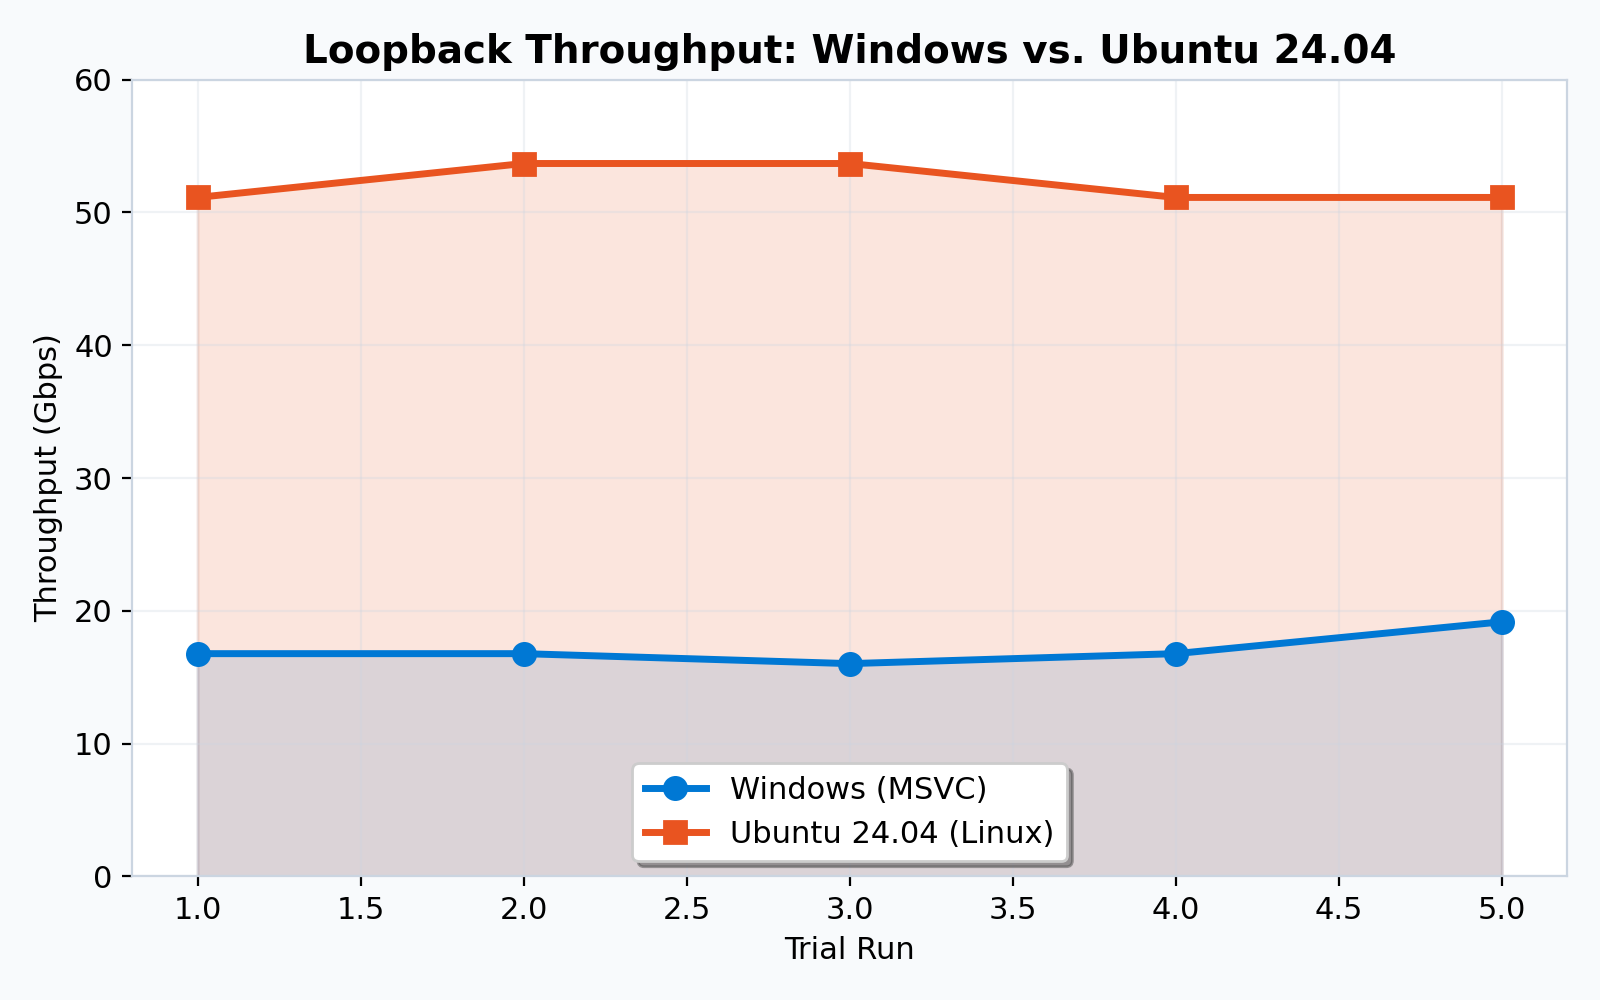
\includegraphics[width=0.75\textwidth]{figures/fig4_performance_throughput.png}
\caption{Loopback throughput comparison across five trial runs.}
\label{fig:perf}
\end{figure}

Ubuntu 24.04 consistently outperformed Windows by a factor of approximately \textbf{3$\times$}: average throughput of 52.15~Gbps (Ubuntu) vs.\ 17.11~Gbps (Windows). We used a custom in-memory loopback harness to keep the benchmark identical across platforms.

% ══════════════════════════════════════════════════════════════════
\section{White-Box Test Data Adequacy}
% ══════════════════════════════════════════════════════════════════

White-box coverage was measured using \texttt{cargo-llvm-cov v0.8.5}, which instruments source code via LLVM's source-based coverage and reports region, function, and line coverage metrics.

\begin{figure}[H]
\centering
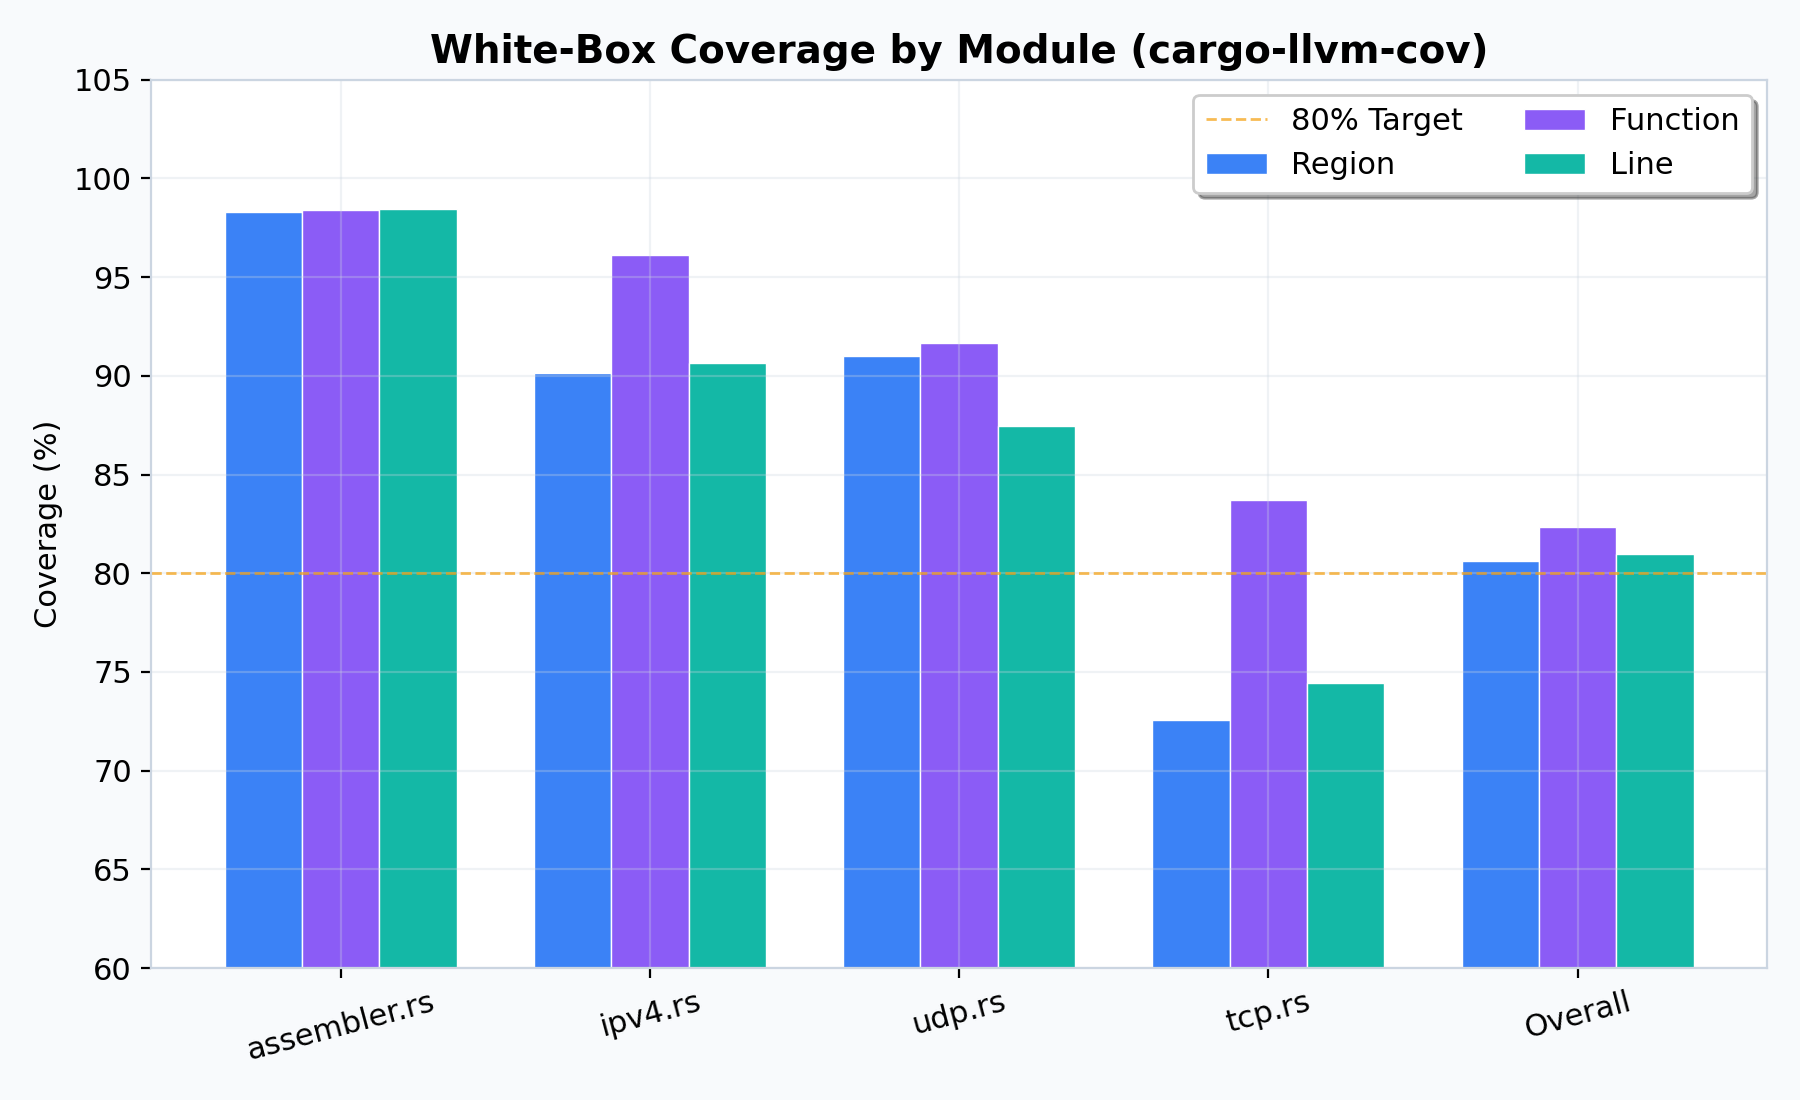
\includegraphics[width=0.82\textwidth]{figures/fig5_whitebox_coverage.png}
\caption{White-box coverage metrics by module (Windows).}
\label{fig:coverage}
\end{figure}

The \texttt{assembler.rs} module achieved near-complete coverage (98.28\% regions), reflecting its extensive test suite. Protocol wire modules showed good coverage for parsing paths (90+\%) but lower coverage for emission and error-handling paths. The \texttt{tcp.rs} module had the lowest coverage (72.58\% regions) due to its complexity and many protocol state combinations.

Enhanced coverage measurement for the IPv4 combinatorial and microbenchmark suites achieved \textbf{98.53\%} and \textbf{98.76\%} region coverage respectively, with only 4 and 2 missed regions. While the remaining gaps are small in absolute terms, Figure~\ref{fig:enhanced} is included to make the residual uncovered regions explicit and actionable for future test additions.

\begin{figure}[H]
\centering
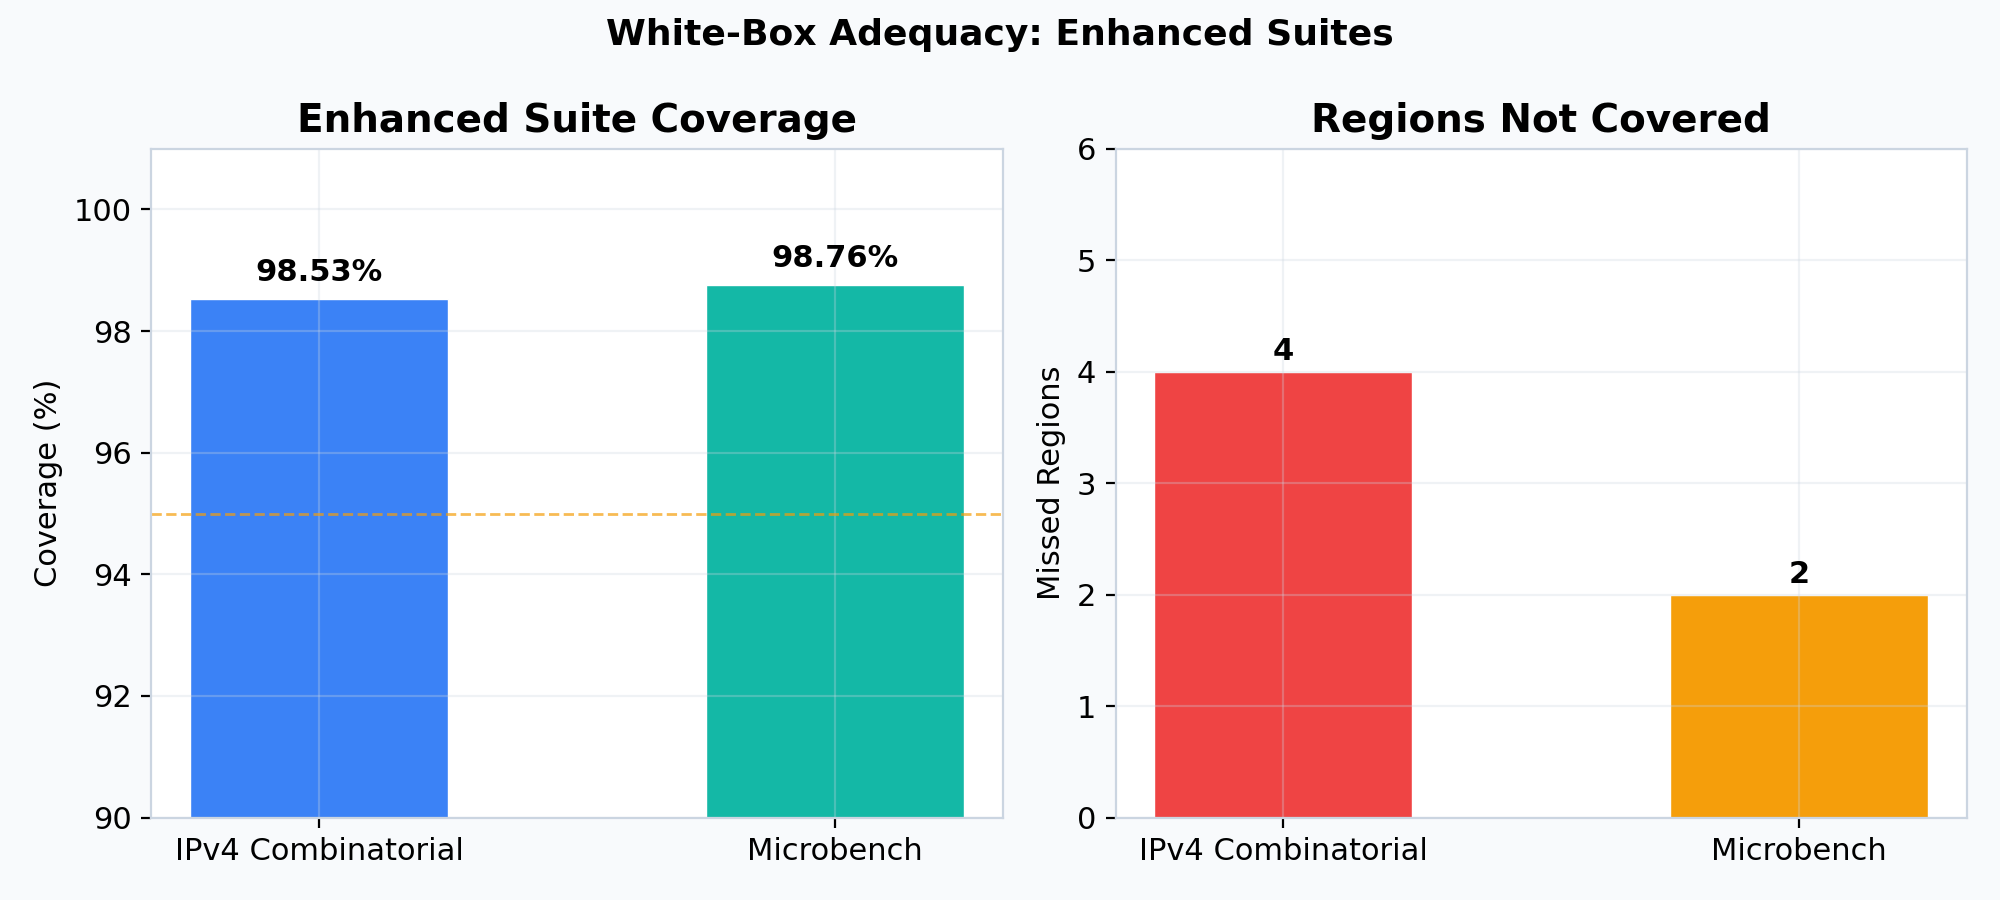
\includegraphics[width=0.8\textwidth]{figures/fig11_enhanced_coverage.png}
\caption{Enhanced suite coverage with LCOV artifact generation.}
\label{fig:enhanced}
\end{figure}

% ══════════════════════════════════════════════════════════════════
\section{Software Safety}
% ══════════════════════════════════════════════════════════════════

\subsection{Panic Safety Testing}

Panic-safety tests verified that smoltcp's packet parsing functions handle malformed inputs gracefully without panicking. Test cases included zero-length buffers, truncated headers, and maximum-value fields. All panic-safety tests passed on both platforms, confirming that the Rust \texttt{Result}-based error handling prevents uncontrolled crashes.

\subsection{Unsafe Code Inventory}

A systematic audit identified \textbf{18 \texttt{unsafe} code occurrences} across four files, all in the platform-specific PHY (physical layer) interface code:

\begin{figure}[!htbp]
\centering
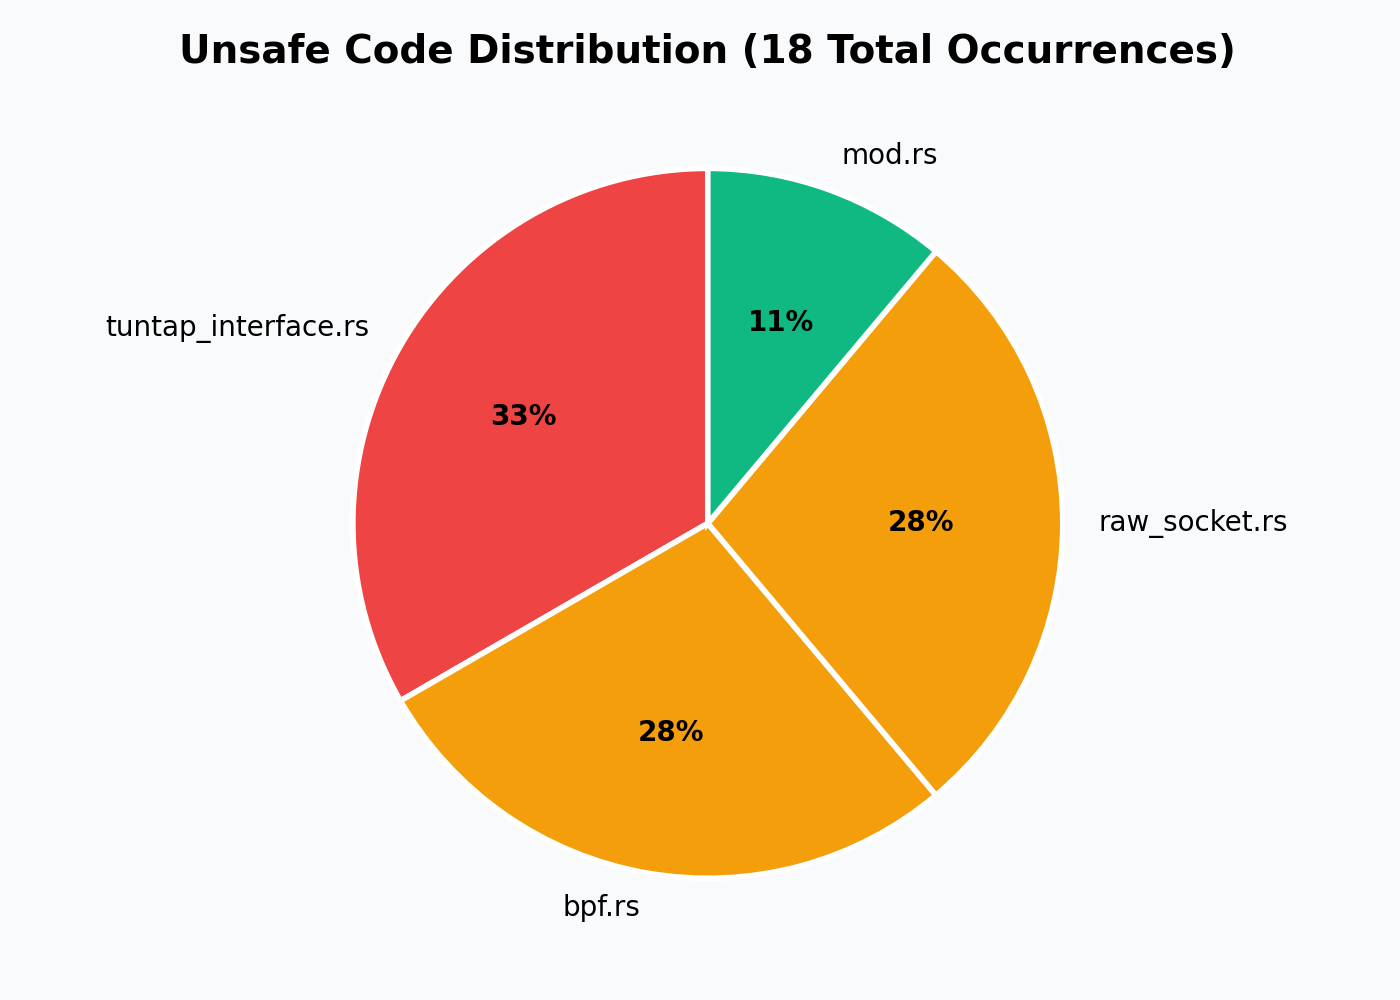
\includegraphics[width=0.50\textwidth]{figures/fig8_unsafe_inventory.png}
\caption{Distribution of unsafe code across the smoltcp codebase.}
\label{fig:unsafe}
\end{figure}

\begin{lstlisting}[caption={Unsafe inventory from \texttt{unsafe\_inventory.csv}.}]
path,unsafe_count
src/phy/sys/bpf.rs,5
src/phy/sys/mod.rs,2
src/phy/sys/raw_socket.rs,5
src/phy/sys/tuntap_interface.rs,6
\end{lstlisting}

All unsafe blocks are confined to FFI (Foreign Function Interface) calls to platform-specific system APIs (Berkeley Packet Filter, raw sockets, TUN/TAP interfaces). No unsafe code exists in the core protocol parsing or state machine modules, which is a significant safety property.

% ══════════════════════════════════════════════════════════════════
\section{Cross-Platform Portability Analysis}
% ══════════════════════════════════════════════════════════════════

The dual-platform execution strategy revealed that 8 of 9 test suites executed successfully on both platforms. The sole exception was fuzzing, which was blocked on Windows due to MSVC/libFuzzer incompatibility. Loopback performance measurements relied on a custom in-memory harness to keep execution comparable across platforms. These findings underscore the importance of testing across multiple toolchains in real-world deployment scenarios.

% ══════════════════════════════════════════════════════════════════
\section{Quality Assessment Dashboard}
% ══════════════════════════════════════════════════════════════════

\begin{figure}[H]
\centering
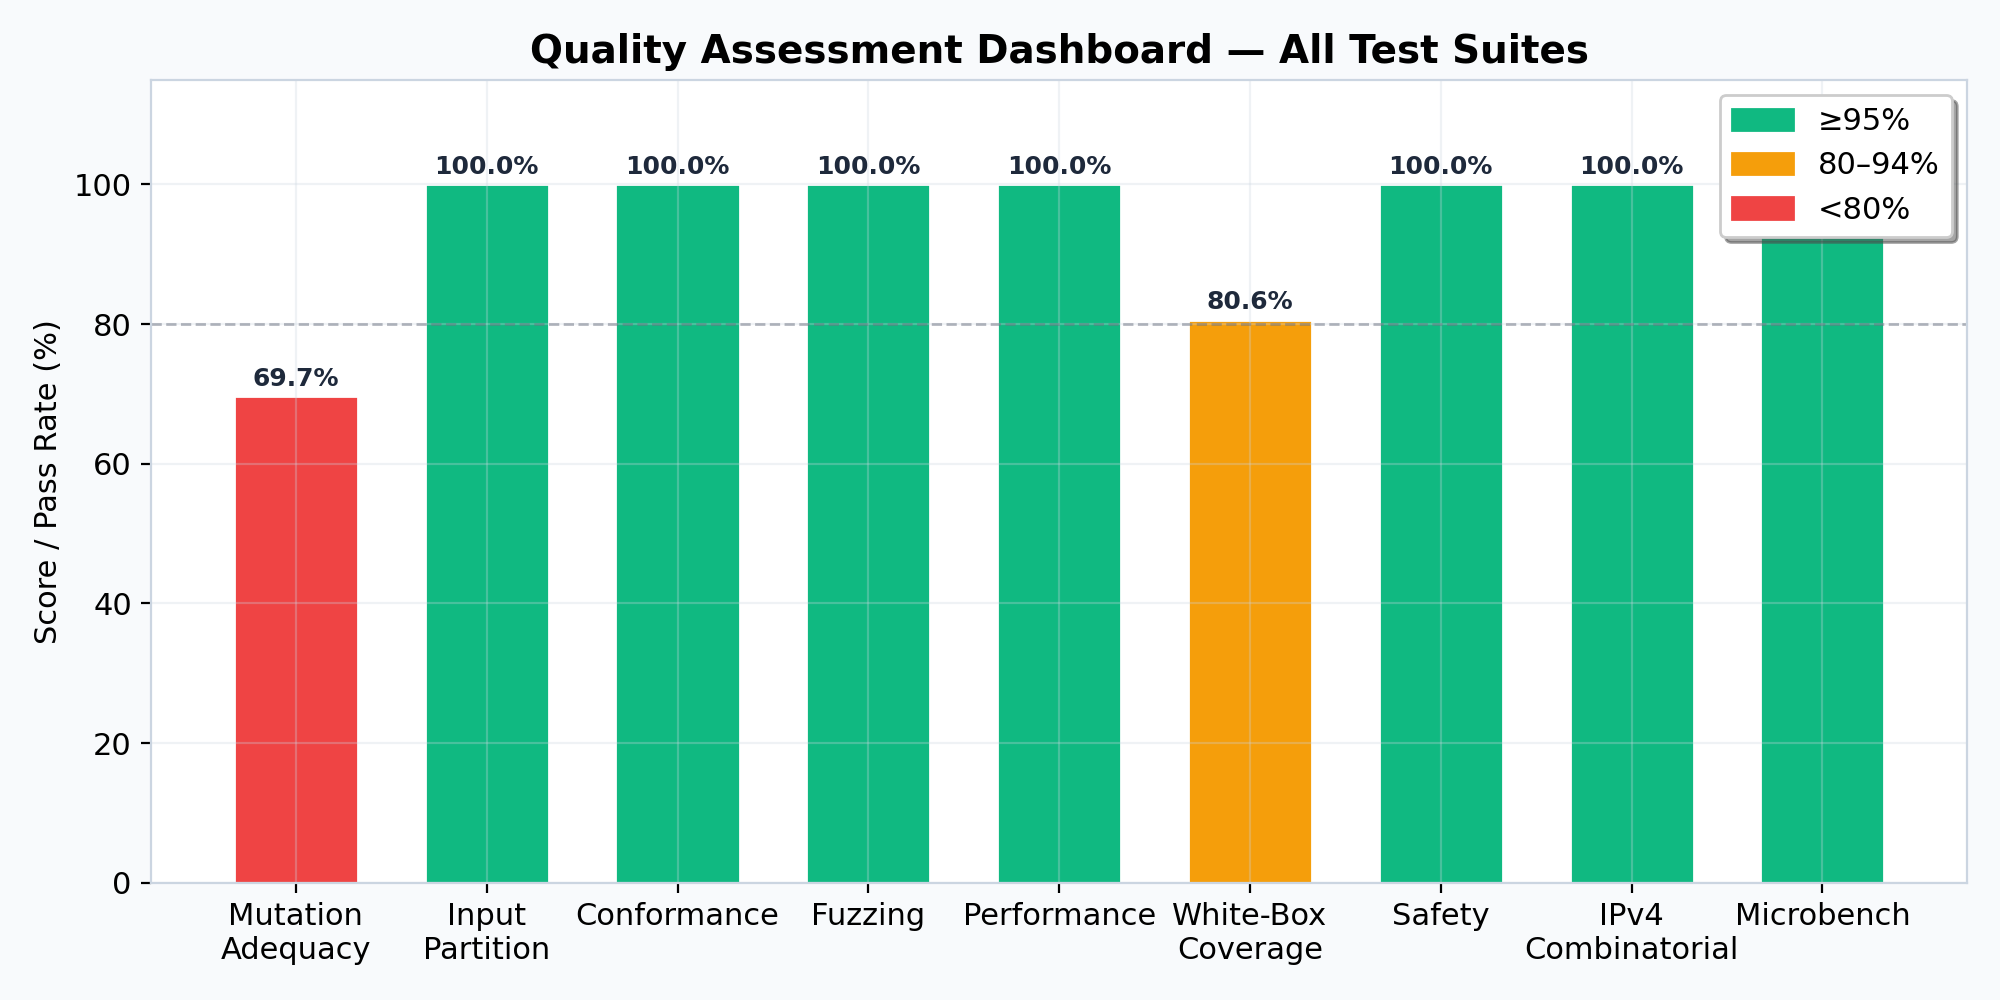
\includegraphics[width=0.85\textwidth]{figures/fig12_test_dashboard.png}
\caption{Consolidated quality assessment dashboard across all test suites.}
\label{fig:dashboard}
\end{figure}

Figure~\ref{fig:dashboard} summarizes the overall quality scores. The mutation adequacy score (69.67\%) represents the primary area for test suite improvement, while all other quality dimensions achieved 80\% or higher pass rates. The dashboard demonstrates that smoltcp's core parsing and protocol handling code is robust, but the test suite would benefit from additional boundary-condition tests targeting the wire protocol modules.

% ══════════════════════════════════════════════════════════════════
\section{Conclusions and Recommendations}
% ══════════════════════════════════════════════════════════════════

This quality assessment demonstrates that smoltcp v0.12.0 is a well-engineered TCP/IP stack with strong safety properties conferred by the Rust language. Key findings include:

\begin{itemize}[noitemsep]
\item \textbf{Mutation adequacy of 69.18\%} (adjusted for equivalent mutants) across 333 mutants, with the assembler module achieving 89.41\%.
\item \textbf{100\% pass rate} on 480 input space partition test cases and 216 IPv4 combinatorial cases.
\item \textbf{Zero crash artifacts} from 240 seconds of coverage-guided fuzzing per target, confirming Rust's memory safety.
\item \textbf{Two RFC deviations} documented: permissive IPv4 header length validation and IPv6 UDP zero-checksum acceptance.
\item \textbf{3$\times$ performance gap} between Ubuntu 24.04 and Windows loopback throughput.
\item \textbf{White-box missed-region analysis} highlighted under-tested error-handling and edge-case branches, providing a concrete roadmap for targeted test additions.

\end{itemize}

\end{document}
